% Graphic for TeX using PGF
% Title: /home/satenske/cours/AP/obj3/TD1/2.dia
% Creator: Dia v0.97.1
% CreationDate: Thu Oct 20 08:54:32 2011
% For: satenske
% \usepackage{tikz}
% The following commands are not supported in PSTricks at present
% We define them conditionally, so when they are implemented,
% this pgf file will use them.
\ifx\du\undefined
  \newlength{\du}
\fi
\setlength{\du}{15\unitlength}
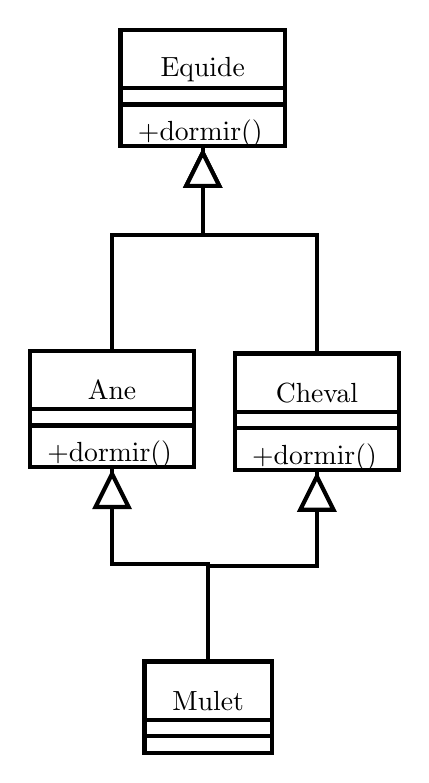
\begin{tikzpicture}
\pgftransformxscale{1.000000}
\pgftransformyscale{-1.000000}
\definecolor{dialinecolor}{rgb}{0.000000, 0.000000, 0.000000}
\pgfsetstrokecolor{dialinecolor}
\definecolor{dialinecolor}{rgb}{1.000000, 1.000000, 1.000000}
\pgfsetfillcolor{dialinecolor}
\pgfsetlinewidth{0.100000\du}
\pgfsetdash{}{0pt}
\definecolor{dialinecolor}{rgb}{1.000000, 1.000000, 1.000000}
\pgfsetfillcolor{dialinecolor}
\fill (18.150000\du,2.250000\du)--(18.150000\du,3.650000\du)--(22.115000\du,3.650000\du)--(22.115000\du,2.250000\du)--cycle;
\definecolor{dialinecolor}{rgb}{0.000000, 0.000000, 0.000000}
\pgfsetstrokecolor{dialinecolor}
\draw (18.150000\du,2.250000\du)--(18.150000\du,3.650000\du)--(22.115000\du,3.650000\du)--(22.115000\du,2.250000\du)--cycle;
% setfont left to latex
\definecolor{dialinecolor}{rgb}{0.000000, 0.000000, 0.000000}
\pgfsetstrokecolor{dialinecolor}
\node at (20.132500\du,3.200000\du){Equide};
\definecolor{dialinecolor}{rgb}{1.000000, 1.000000, 1.000000}
\pgfsetfillcolor{dialinecolor}
\fill (18.150000\du,3.650000\du)--(18.150000\du,4.050000\du)--(22.115000\du,4.050000\du)--(22.115000\du,3.650000\du)--cycle;
\definecolor{dialinecolor}{rgb}{0.000000, 0.000000, 0.000000}
\pgfsetstrokecolor{dialinecolor}
\draw (18.150000\du,3.650000\du)--(18.150000\du,4.050000\du)--(22.115000\du,4.050000\du)--(22.115000\du,3.650000\du)--cycle;
\definecolor{dialinecolor}{rgb}{1.000000, 1.000000, 1.000000}
\pgfsetfillcolor{dialinecolor}
\fill (18.150000\du,4.050000\du)--(18.150000\du,5.050000\du)--(22.115000\du,5.050000\du)--(22.115000\du,4.050000\du)--cycle;
\definecolor{dialinecolor}{rgb}{0.000000, 0.000000, 0.000000}
\pgfsetstrokecolor{dialinecolor}
\draw (18.150000\du,4.050000\du)--(18.150000\du,5.050000\du)--(22.115000\du,5.050000\du)--(22.115000\du,4.050000\du)--cycle;
% setfont left to latex
\definecolor{dialinecolor}{rgb}{0.000000, 0.000000, 0.000000}
\pgfsetstrokecolor{dialinecolor}
\node[anchor=west] at (18.300000\du,4.750000\du){+dormir()};
\pgfsetlinewidth{0.100000\du}
\pgfsetdash{}{0pt}
\definecolor{dialinecolor}{rgb}{1.000000, 1.000000, 1.000000}
\pgfsetfillcolor{dialinecolor}
\fill (20.900000\du,10.050000\du)--(20.900000\du,11.450000\du)--(24.865000\du,11.450000\du)--(24.865000\du,10.050000\du)--cycle;
\definecolor{dialinecolor}{rgb}{0.000000, 0.000000, 0.000000}
\pgfsetstrokecolor{dialinecolor}
\draw (20.900000\du,10.050000\du)--(20.900000\du,11.450000\du)--(24.865000\du,11.450000\du)--(24.865000\du,10.050000\du)--cycle;
% setfont left to latex
\definecolor{dialinecolor}{rgb}{0.000000, 0.000000, 0.000000}
\pgfsetstrokecolor{dialinecolor}
\node at (22.882500\du,11.000000\du){Cheval};
\definecolor{dialinecolor}{rgb}{1.000000, 1.000000, 1.000000}
\pgfsetfillcolor{dialinecolor}
\fill (20.900000\du,11.450000\du)--(20.900000\du,11.850000\du)--(24.865000\du,11.850000\du)--(24.865000\du,11.450000\du)--cycle;
\definecolor{dialinecolor}{rgb}{0.000000, 0.000000, 0.000000}
\pgfsetstrokecolor{dialinecolor}
\draw (20.900000\du,11.450000\du)--(20.900000\du,11.850000\du)--(24.865000\du,11.850000\du)--(24.865000\du,11.450000\du)--cycle;
\definecolor{dialinecolor}{rgb}{1.000000, 1.000000, 1.000000}
\pgfsetfillcolor{dialinecolor}
\fill (20.900000\du,11.850000\du)--(20.900000\du,12.850000\du)--(24.865000\du,12.850000\du)--(24.865000\du,11.850000\du)--cycle;
\definecolor{dialinecolor}{rgb}{0.000000, 0.000000, 0.000000}
\pgfsetstrokecolor{dialinecolor}
\draw (20.900000\du,11.850000\du)--(20.900000\du,12.850000\du)--(24.865000\du,12.850000\du)--(24.865000\du,11.850000\du)--cycle;
% setfont left to latex
\definecolor{dialinecolor}{rgb}{0.000000, 0.000000, 0.000000}
\pgfsetstrokecolor{dialinecolor}
\node[anchor=west] at (21.050000\du,12.550000\du){+dormir()};
\pgfsetlinewidth{0.100000\du}
\pgfsetdash{}{0pt}
\definecolor{dialinecolor}{rgb}{1.000000, 1.000000, 1.000000}
\pgfsetfillcolor{dialinecolor}
\fill (15.965000\du,9.985000\du)--(15.965000\du,11.385000\du)--(19.930000\du,11.385000\du)--(19.930000\du,9.985000\du)--cycle;
\definecolor{dialinecolor}{rgb}{0.000000, 0.000000, 0.000000}
\pgfsetstrokecolor{dialinecolor}
\draw (15.965000\du,9.985000\du)--(15.965000\du,11.385000\du)--(19.930000\du,11.385000\du)--(19.930000\du,9.985000\du)--cycle;
% setfont left to latex
\definecolor{dialinecolor}{rgb}{0.000000, 0.000000, 0.000000}
\pgfsetstrokecolor{dialinecolor}
\node at (17.947500\du,10.935000\du){Ane};
\definecolor{dialinecolor}{rgb}{1.000000, 1.000000, 1.000000}
\pgfsetfillcolor{dialinecolor}
\fill (15.965000\du,11.385000\du)--(15.965000\du,11.785000\du)--(19.930000\du,11.785000\du)--(19.930000\du,11.385000\du)--cycle;
\definecolor{dialinecolor}{rgb}{0.000000, 0.000000, 0.000000}
\pgfsetstrokecolor{dialinecolor}
\draw (15.965000\du,11.385000\du)--(15.965000\du,11.785000\du)--(19.930000\du,11.785000\du)--(19.930000\du,11.385000\du)--cycle;
\definecolor{dialinecolor}{rgb}{1.000000, 1.000000, 1.000000}
\pgfsetfillcolor{dialinecolor}
\fill (15.965000\du,11.785000\du)--(15.965000\du,12.785000\du)--(19.930000\du,12.785000\du)--(19.930000\du,11.785000\du)--cycle;
\definecolor{dialinecolor}{rgb}{0.000000, 0.000000, 0.000000}
\pgfsetstrokecolor{dialinecolor}
\draw (15.965000\du,11.785000\du)--(15.965000\du,12.785000\du)--(19.930000\du,12.785000\du)--(19.930000\du,11.785000\du)--cycle;
% setfont left to latex
\definecolor{dialinecolor}{rgb}{0.000000, 0.000000, 0.000000}
\pgfsetstrokecolor{dialinecolor}
\node[anchor=west] at (16.115000\du,12.485000\du){+dormir()};
\pgfsetlinewidth{0.100000\du}
\pgfsetdash{}{0pt}
\definecolor{dialinecolor}{rgb}{1.000000, 1.000000, 1.000000}
\pgfsetfillcolor{dialinecolor}
\fill (18.730000\du,17.470000\du)--(18.730000\du,18.870000\du)--(21.795000\du,18.870000\du)--(21.795000\du,17.470000\du)--cycle;
\definecolor{dialinecolor}{rgb}{0.000000, 0.000000, 0.000000}
\pgfsetstrokecolor{dialinecolor}
\draw (18.730000\du,17.470000\du)--(18.730000\du,18.870000\du)--(21.795000\du,18.870000\du)--(21.795000\du,17.470000\du)--cycle;
% setfont left to latex
\definecolor{dialinecolor}{rgb}{0.000000, 0.000000, 0.000000}
\pgfsetstrokecolor{dialinecolor}
\node at (20.262500\du,18.420000\du){Mulet};
\definecolor{dialinecolor}{rgb}{1.000000, 1.000000, 1.000000}
\pgfsetfillcolor{dialinecolor}
\fill (18.730000\du,18.870000\du)--(18.730000\du,19.270000\du)--(21.795000\du,19.270000\du)--(21.795000\du,18.870000\du)--cycle;
\definecolor{dialinecolor}{rgb}{0.000000, 0.000000, 0.000000}
\pgfsetstrokecolor{dialinecolor}
\draw (18.730000\du,18.870000\du)--(18.730000\du,19.270000\du)--(21.795000\du,19.270000\du)--(21.795000\du,18.870000\du)--cycle;
\definecolor{dialinecolor}{rgb}{1.000000, 1.000000, 1.000000}
\pgfsetfillcolor{dialinecolor}
\fill (18.730000\du,19.270000\du)--(18.730000\du,19.670000\du)--(21.795000\du,19.670000\du)--(21.795000\du,19.270000\du)--cycle;
\definecolor{dialinecolor}{rgb}{0.000000, 0.000000, 0.000000}
\pgfsetstrokecolor{dialinecolor}
\draw (18.730000\du,19.270000\du)--(18.730000\du,19.670000\du)--(21.795000\du,19.670000\du)--(21.795000\du,19.270000\du)--cycle;
\pgfsetlinewidth{0.100000\du}
\pgfsetdash{}{0pt}
\pgfsetmiterjoin
\pgfsetbuttcap
{
\definecolor{dialinecolor}{rgb}{0.000000, 0.000000, 0.000000}
\pgfsetfillcolor{dialinecolor}
% was here!!!
\definecolor{dialinecolor}{rgb}{0.000000, 0.000000, 0.000000}
\pgfsetstrokecolor{dialinecolor}
\draw (20.132500\du,5.099988\du)--(20.132500\du,7.200000\du)--(22.882500\du,7.200000\du)--(22.882500\du,10.000476\du);
}
\definecolor{dialinecolor}{rgb}{0.000000, 0.000000, 0.000000}
\pgfsetstrokecolor{dialinecolor}
\draw (20.132500\du,6.011791\du)--(20.132500\du,7.200000\du)--(22.882500\du,7.200000\du)--(22.882500\du,10.000476\du);
\pgfsetmiterjoin
\definecolor{dialinecolor}{rgb}{1.000000, 1.000000, 1.000000}
\pgfsetfillcolor{dialinecolor}
\fill (20.532500\du,6.011791\du)--(20.132500\du,5.211791\du)--(19.732500\du,6.011791\du)--cycle;
\pgfsetlinewidth{0.100000\du}
\pgfsetdash{}{0pt}
\pgfsetmiterjoin
\definecolor{dialinecolor}{rgb}{0.000000, 0.000000, 0.000000}
\pgfsetstrokecolor{dialinecolor}
\draw (20.532500\du,6.011791\du)--(20.132500\du,5.211791\du)--(19.732500\du,6.011791\du)--cycle;
% setfont left to latex
\pgfsetlinewidth{0.100000\du}
\pgfsetdash{}{0pt}
\pgfsetmiterjoin
\pgfsetbuttcap
{
\definecolor{dialinecolor}{rgb}{0.000000, 0.000000, 0.000000}
\pgfsetfillcolor{dialinecolor}
% was here!!!
\definecolor{dialinecolor}{rgb}{0.000000, 0.000000, 0.000000}
\pgfsetstrokecolor{dialinecolor}
\draw (20.132500\du,5.099988\du)--(20.132500\du,7.200000\du)--(17.947500\du,7.200000\du)--(17.947500\du,9.936189\du);
}
\definecolor{dialinecolor}{rgb}{0.000000, 0.000000, 0.000000}
\pgfsetstrokecolor{dialinecolor}
\draw (20.132500\du,6.011791\du)--(20.132500\du,7.200000\du)--(17.947500\du,7.200000\du)--(17.947500\du,9.936189\du);
\pgfsetmiterjoin
\definecolor{dialinecolor}{rgb}{1.000000, 1.000000, 1.000000}
\pgfsetfillcolor{dialinecolor}
\fill (20.532500\du,6.011791\du)--(20.132500\du,5.211791\du)--(19.732500\du,6.011791\du)--cycle;
\pgfsetlinewidth{0.100000\du}
\pgfsetdash{}{0pt}
\pgfsetmiterjoin
\definecolor{dialinecolor}{rgb}{0.000000, 0.000000, 0.000000}
\pgfsetstrokecolor{dialinecolor}
\draw (20.532500\du,6.011791\du)--(20.132500\du,5.211791\du)--(19.732500\du,6.011791\du)--cycle;
% setfont left to latex
\pgfsetlinewidth{0.100000\du}
\pgfsetdash{}{0pt}
\pgfsetmiterjoin
\pgfsetbuttcap
{
\definecolor{dialinecolor}{rgb}{0.000000, 0.000000, 0.000000}
\pgfsetfillcolor{dialinecolor}
% was here!!!
\definecolor{dialinecolor}{rgb}{0.000000, 0.000000, 0.000000}
\pgfsetstrokecolor{dialinecolor}
\draw (22.882500\du,12.900354\du)--(22.882500\du,15.160037\du)--(20.262500\du,15.160037\du)--(20.262500\du,17.419719\du);
}
\definecolor{dialinecolor}{rgb}{0.000000, 0.000000, 0.000000}
\pgfsetstrokecolor{dialinecolor}
\draw (22.882500\du,13.812157\du)--(22.882500\du,15.160037\du)--(20.262500\du,15.160037\du)--(20.262500\du,17.419719\du);
\pgfsetmiterjoin
\definecolor{dialinecolor}{rgb}{1.000000, 1.000000, 1.000000}
\pgfsetfillcolor{dialinecolor}
\fill (23.282500\du,13.812157\du)--(22.882500\du,13.012157\du)--(22.482500\du,13.812157\du)--cycle;
\pgfsetlinewidth{0.100000\du}
\pgfsetdash{}{0pt}
\pgfsetmiterjoin
\definecolor{dialinecolor}{rgb}{0.000000, 0.000000, 0.000000}
\pgfsetstrokecolor{dialinecolor}
\draw (23.282500\du,13.812157\du)--(22.882500\du,13.012157\du)--(22.482500\du,13.812157\du)--cycle;
% setfont left to latex
\pgfsetlinewidth{0.100000\du}
\pgfsetdash{}{0pt}
\pgfsetmiterjoin
\pgfsetbuttcap
{
\definecolor{dialinecolor}{rgb}{0.000000, 0.000000, 0.000000}
\pgfsetfillcolor{dialinecolor}
% was here!!!
\definecolor{dialinecolor}{rgb}{0.000000, 0.000000, 0.000000}
\pgfsetstrokecolor{dialinecolor}
\draw (17.947500\du,12.835354\du)--(17.947500\du,15.127537\du)--(20.262500\du,15.127537\du)--(20.262500\du,17.419719\du);
}
\definecolor{dialinecolor}{rgb}{0.000000, 0.000000, 0.000000}
\pgfsetstrokecolor{dialinecolor}
\draw (17.947500\du,13.747157\du)--(17.947500\du,15.127537\du)--(20.262500\du,15.127537\du)--(20.262500\du,17.419719\du);
\pgfsetmiterjoin
\definecolor{dialinecolor}{rgb}{1.000000, 1.000000, 1.000000}
\pgfsetfillcolor{dialinecolor}
\fill (18.347500\du,13.747157\du)--(17.947500\du,12.947157\du)--(17.547500\du,13.747157\du)--cycle;
\pgfsetlinewidth{0.100000\du}
\pgfsetdash{}{0pt}
\pgfsetmiterjoin
\definecolor{dialinecolor}{rgb}{0.000000, 0.000000, 0.000000}
\pgfsetstrokecolor{dialinecolor}
\draw (18.347500\du,13.747157\du)--(17.947500\du,12.947157\du)--(17.547500\du,13.747157\du)--cycle;
% setfont left to latex
\end{tikzpicture}
